\documentclass[11pt]{amsart}
\usepackage{geometry}           % See geometry.pdf to learn the layout options. There are lots.
\geometry{letterpaper} % ... or a4paper or a5paper  or ... 
%\geometry{landscape}                % Activate for for rotated page geometry
%\usepackage[parfill]{parskip}    % Activate to begin paragraphs with an empty line rather than an
%indent
\usepackage{graphicx}
\usepackage{amssymb}
\usepackage{epstopdf}
\usepackage{amsmath}
\DeclareGraphicsRule{.tif}{png}{.png}{`convert #1 `dirname #1`/`basename #1 .tif`.png}

\title{Applying the Henyey method to tidally induced stellar oscillations}
\author{Andrew Bunting}
%\date{}                                           % Activate to display a given date or no date
%
\begin{document}

\maketitle

\section{Introduction}

This is an explanation, record and walkthrough of the derivation and origin of the equations used in the code to solve the stellar oscillation equations using the Henyey method.  Initially the discussion will be fairly abstract and general, but this will become more and more specific as we go along.

To start with, we will address the structure of the method overall, to get a feel for the big picture to try to avoid getting bogged down in details.  Then we will move through the relevant sections of the method in sequence, first with the recurrence relations for $\underline{\alpha}$ and $\vec{\gamma}$; we will then discuss the application of the outer boundary conditions; after that we will discuss the recurrence relation for $\vec{u}$ and $\vec{v}$; finishing off with a discussion of practicalities, such as minimising the amount of memory needed.


\section{Overall structure}

To start with, the structure of the equations must be set out.  This method is used to solve four linear, first order differential equations.  Whilst it is not necessary in general, here we will be restricting ourselves to the case where the two pairs of variables are on a staggered grid, with $\vec{u}$ being evaluated at the outer edge of the cell, and $\vec{v}$ being evaluated at the centre of the cell, where $\vec{u} = \left( a, b \right)^{T}$ and $\vec{v} = \left( c, d \right)^{T}$

The boundary equations are split, two apply at the centre ($\vec{u} = 0$) and two apply at the surface of the star.  Because of this, it is difficult to work with a solution from one boundary to the other, as the problem is under-constrained until all boundary conditions can be applied.

In order to get around this, the Henyey method uses a two-stage approach.  A relation between $\vec{u}$ and $\vec{v}$ is used, which is formulated in such a way that conditions upon the coefficients can be found which reproduce the central boundary condition.  This relation is

\begin{equation} \label{eq:relation}
\vec{u}_{k}  + \underline{\alpha}_{k}  \vec{v}_{k}  + \vec{\gamma}_{k}  = 0,
\end{equation}
\\
which obeys the central boundary condition if $\underline{\alpha}_{0} = 0$ and $\vec{\gamma}_{0} = 0$ are used as a surrogate.  Recurrence relations for the coefficients in this equation ($\underline{\alpha}$ and $\vec{\gamma}$) are used to calculate the values of these coefficients at each point, including at the surface.  Using the surface boundary conditions with the outermost coefficients, the values for $\vec{u}$ and $\vec{v}$ can be evaluated.  Then, another recurrence relation can be found, which relates the values of $\underline{\alpha}$, $\vec{\gamma}$, $\vec{u}$ and $\vec{v}$ at a given point, to the values of $\vec{u}$ and $\vec{v}$ at the adjacent point just inside.  This enables them to be evaluated at all points throughout the star, and the solution is complete.

To describe this problem more specifically, we must look at the structure of the equations in question, and the variables involved.  Two equations involve the derivative of $\vec{u}$ but not $\vec{v}$, and the other two include the derivative of $\vec{v}$ but not $\vec{u}$.  Because of this, we can split the four equations into two matrix equations:

\begin{equation} \label{eq:ACD}
\underline{A}_{k,k+1} \vec{u}_{k} + \underline{C}_{k,k+1} \vec{u}_{k+1} + \underline{D}_{k,k+1} \vec{v}_{k+1} = \vec{M}_{k,k+1},
\end{equation} 

\begin{equation} \label{eq:EFH}
\underline{E}_{k,k+1} \vec{u}_{k} + \underline{F}_{k,k+1} \vec{v}_{k} + \underline{H}_{k,k+1} \vec{v}_{k+1} = \vec{N}_{k,k+1}.
\end{equation} 
\\

This structure means that the two equations with derivatives of $\vec{u}$ make up equation \ref{eq:ACD}, which is evaluated at the midpoint of cell $k+1$; and the two equations with derivatives of $\vec{v}$ make up equation \ref{eq:EFH}, which is evaluated at the outer edge of cell k.  Notably, this structure ensures that the matrices B and G, which would be included in a more general formulation, are ignored from the start, as they would be null at all points, which helps to avoid issues like trying to invert a singular matrix.


\begin{figure}
\begin{center}
\label{fig:overview}
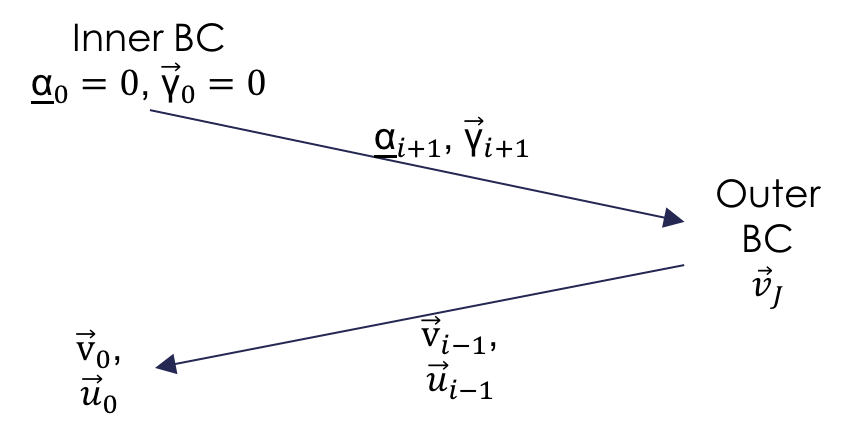
\includegraphics[width = 0.5 \textwidth]{Overview.png}
\caption{A diagrammatic overview of the Henyey method, showing what is being evaluated at each stage of the code.}
\end{center}
\end{figure}



\section{$\underline{\alpha}$ and $\vec{\gamma}$ recurrence relations}

The relation $\vec{u} + \underline{\alpha} \vec{v} + \vec{\gamma} = 0$ is formulated this way as it enables the central boundary condition to be re-expressed as $\underline{\alpha} = 0$ and $\vec{\gamma} = 0$ at the centre.  By combining this initial condition with a recurrence relation, we can iterate outwards to find their values at all points in the star.

There are many different ways to formulate the recurrence relation, some of which will be shown in the following sub-sections.  The relevant equations are equations \ref{eq:relation}, \ref{eq:ACD} and \ref{eq:EFH}.  The key idea is to use these equations to reflect the structure of equation \ref{eq:relation}, evaluated at $k+1$, and to compare coefficients in order to get the equations for $\underline{\alpha}_{k+1}$ and $\vec{\gamma}_{k+1}$.

For ease of reading, the subscripts on the coefficients in equations \ref{eq:ACD} and \ref{eq:EFH} will be dropped, but the $k,k+1$ subscripts are implied, and any other subscripts will be explicitly stated.

\subsection{Method I}

Use equation \ref{eq:relation} to substitute for $\vec{u}_{k}$ in equations \ref{eq:ACD} and \ref{eq:EFH}.

\begin{equation} \label{eq:Ia}
\vec{u}_{k}  = - \underline{\alpha}_{k}  \vec{v}_{k}  - \vec{\gamma}_{k},
\end{equation}
\\
which leads to

\begin{equation} \label{eq:Ib}
- \underline{A} \left(  \underline{\alpha}_{k}  \vec{v}_{k}  + \vec{\gamma}_{k} \right) + \underline{C} \vec{u}_{k+1} + \underline{D} \vec{v}_{k+1} = \vec{M}      \longrightarrow       - \underline{A} \, \underline{\alpha}_{k}  \vec{v}_{k}  + \underline{C} \vec{u}_{k+1} + \underline{D} \vec{v}_{k+1} = \vec{M}  + \underline{A} \vec{\gamma}_{k},
\end{equation} 

\begin{equation} \label{eq:Ic}
- \underline{E} \left(  \underline{\alpha}_{k}  \vec{v}_{k}  + \vec{\gamma}_{k} \right) + \underline{F} \vec{v}_{k} + \underline{H} \vec{v}_{k+1} = \vec{N}   \longrightarrow   \left( \underline{F} - \underline{E} \, \underline{\alpha}_{k} \right) \vec{v}_{k} + \underline{H} \vec{v}_{k+1} = \vec{N} + \underline{E} \vec{\gamma}_{k.}
\end{equation} 
\\
We then isolate $-\vec{v}_{k}$ in equation \ref{eq:Ib} and $\vec{v}_{k}$ in equation \ref{eq:Ic}, giving

\begin{equation} \label{eq:Id}
- \underline{A} \left(  \underline{\alpha}_{k}  \vec{v}_{k}  + \vec{\gamma}_{k} \right) + \underline{C} \vec{u}_{k+1} + \underline{D} \vec{v}_{k+1} = \vec{M}      \longrightarrow       - \underline{A} \, \underline{\alpha}_{k}  \vec{v}_{k}  + \underline{C} \vec{u}_{k+1} + \underline{D} \vec{v}_{k+1} = \vec{M}  + \underline{A} \vec{\gamma}_{k},
\end{equation} 

\begin{equation} \label{eq:Ie}
- \underline{E} \left(  \underline{\alpha}_{k}  \vec{v}_{k}  + \vec{\gamma}_{k} \right) + \underline{F} \vec{v}_{k} + \underline{H} \vec{v}_{k+1} = \vec{N}   \longrightarrow   \left( \underline{F} - \underline{E} \, \underline{\alpha}_{k} \right) \vec{v}_{k} + \underline{H} \vec{v}_{k+1} = \vec{N} + \underline{E} \vec{\gamma}_{k.}
\end{equation} 
\\

















\subsection{Assumptions}

The equilibrium case is taken to be time-independent (or at least changing on a time-scale much 
smaller than the time-scale of the oscillations), spherically symmetric (therefore equilibrium 
quantities are functions only of the radius, r), and static (such that the fluid velocity of 
equilibrium, $\vec{u}_{0} = 0$).

In this analysis, we will also use the Cowling approximation, which states that the perturbation
to the self-gravity potential is negligible.  Therefore the perturbation to $\Phi$ is given by 
the potential due to the perturbing body, $\Phi_{P}$.



\subsection{Linearising}

To study effects of infinitesimal perturbations to the system, the variables are expanded into
their equilibrium and perturbed components, such as $q = q_{0} + q'$, for some variable, $q$.
The equilibrium quantities themselves satisfy the fluid equations, so cancel out.  Terms which are
second order in perturbed quantities are taken to be negligible, because the perturbation is
taken to be very small. This leaves only terms which are linear in perturbed quantities.

Looking at the perturbed velocity in particular, and recalling that the equilibrium state is taken
to be static, we see that $\vec{u} = 0 + \vec{u}'$.  We can re-express this in terms of $\vec{\xi}$,
 the displacement from equilibrium ($\vec{\xi} = \vec{r} - \vec{r}_{0}$).  Relating the Lagrangian and 
Eulerian descriptions of the perturbed velocity gives:

\begin{equation}
\delta \vec{u} = \vec{u}' + (\vec{\xi} \cdot \vec{\nabla}) \vec{u}_{0} \longrightarrow \delta \vec{u} = \vec{u}'
\end{equation}
\\
which shows that the perturbed velocity is the same in both the Eulerian and Lagrangian descriptions.

We can then use this to relate the displacement to the perturbed velocity, as

\begin{equation}
\delta \vec{u} = \vec{u}(\vec{r}_{0} + \vec{\xi}) - \vec{u}(\vec{r}_{0}) = \frac{d\vec{r}}{dt} - \frac{d\vec{r}_{0}}{dt}
= \frac{d}{dt} \left( \vec{r} - \vec{r}_{0} \right) = \frac{d}{dt} \vec{\xi}
\end{equation}
\\
and as $\delta\vec{u} = \vec{u}'$, we can also say that $\vec{u} = \frac{\partial \vec{\xi}}{\partial t}$.






\subsection{Continuity equation}

The continuity equation is a result from the conservation of mass, and can be expressed as

\begin{equation} \frac{\partial \, \rho}{\partial \, t} + \vec{\nabla} \cdot ( \rho \, \vec{u} )
\end{equation}
\\
where $\rho$ is the density.  This is linearised to

\begin{equation}
\frac{\partial}{\partial t} \left( \rho' + \vec{\nabla} \cdot \left( \rho_{0} \vec{\xi} \right) \right) = 0
\end{equation}
\\
using the fact that the equilibrium quantities are time-independent to bring the partial time
derivative outside the brackets.



\subsection{Momentum equation}

This equation arises from examining the forces acting on a fluid element, given as

\begin{equation} \rho \left( \frac{\partial}{\partial \, t} +  \vec{u} \cdot \vec{\nabla} \right)
\vec{u} = \rho \vec{f} - \vec{\nabla} p - \rho \vec{\nabla} \Phi + \vec{\nabla} \cdot \hat{\Pi}
\end{equation}
\\
where $p$ is the pressure, , $\Phi$ is the gravitational potential, $\vec{f}$ is
the EM and external forces per unit volume, and $\hat{\Pi}$ is the viscous stress tensor. In this
case, $\vec{f}$ and $\hat{\Pi}$ may be neglected, as the fluid is almost an ideal gas, is charge
neutral, and the only external influence is gravitational, which is taken into account by $\Phi$.

Linearising this, we use the Cowling approximation to use the substitution $\Phi = \Phi_{0} + \Phi_{P}$.
This gives

\begin{equation}
\rho_{0} \frac{\partial^{2} \vec{\xi}}{\partial t^{2}} = - \vec{\nabla} p' - \rho_{0} \vec{\nabla} \Phi_{P}
- \rho' \vec{\nabla} \Phi_{0}.
\end{equation}



\subsection{Energy equation}

This equation arises from considering the release and flux of energy and can be expressed as

\begin{equation}
\rho T \left( \frac{\partial}{\partial t} + \vec{u} \cdot \vec{\nabla} \right) s =
\rho \left( \epsilon_{N} + \epsilon_{\nu} \right) - \vec{\nabla} \cdot \vec{F}
\end{equation}
\\
where $s$ is the specific entropy, $\epsilon_{N}$ is the specific nuclear energy generation rate,
$\epsilon_{\nu}$ is the specific rate of release of heat due to viscosity, and $\vec{F}$ is the radiative flux.

In linearising, we neglect both $\epsilon_{N}$ and $\epsilon_{\nu}$, as we expect the nuclear energy
generation rate to be insensitive to the small perturbations (and nuclear energy generation will only
occur in a small region at the core, where oscillations are expected to be smallest) and we are
neglecting viscosity still.

\begin{equation}
\rho_{0} T_{0} \frac{\partial}{\partial t} \left( s' + \vec{\xi} \cdot \vec{\nabla} s_{0} \right)
= s - \vec{\nabla} \cdot \vec{F}.
\end{equation}
\\

\subsection{Associated equations}

These equations are necessary to relate variables to each other, particularly in terms of gradients of
equilibrium quantities.

First, we have the express the radiative flux using the radiative diffusion equation as

\begin{equation}
\vec{F} = - K \vec{\nabla} T
\end{equation}
\\
where $K = \frac{4 a c_{*}}{3 \kappa \rho} T^{3}$, where $a = \frac{4 \sigma}{c_{*}} = 7.5657 \times 10^{-15}$ 
erg cm$^{-3}$ K$^{-4}$ is the radiation density constant ($\sigma$ is the Stefan-Boltzmann constant),
$c_{*}$ is the speed of light (the subscript-asterisk is to differentiate it from the sound speed) 
and $\kappa$ is the opacity.

Linearising will give us

\begin{equation}
\vec{F}' = - K' \vec{\nabla} T_{0} - K_{0} \vec{\nabla} T'
\end{equation}
\\
and

\begin{equation}
\frac{K'}{K_{0}} = 3 \frac{T'}{T_{0}} - \frac{\kappa'}{\kappa_{0}} - \frac{\rho'}{\rho_{0}}.
\end{equation}
\\

We must also find a relation for the change in opacity, the change in density, and the change in specific entropy,
in terms of the variables of state which we are most interested in.  For the most part, this
means expressing total derivatives in terms of $p$ and $T$, but not always -- this is largely
dictated by the derivatives which are available through MESAstar.

For the opacity, we express it as $\kappa = \kappa \left( \ln (\rho) , \ln(T) \right)$, which gives us

\begin{equation}
d\kappa = \left( \frac{\partial \kappa}{\partial \ln \rho} \right)_{T} d(\ln \rho) + \left( \frac{\partial \kappa}{\partial \ln T} \right)_{\rho} d(\ln T)
\end{equation}
\\
which is linearised to give

\begin{equation}
\kappa' = \left( \frac{\partial \kappa}{\partial \ln \rho} \right)_{T} \frac{\rho'}{\rho_{0}} + \left( \frac{\partial \kappa}{\partial \ln T} \right)_{\rho} \frac{T'}{T_{0}}
\end{equation}
\\
which is left in this form, as the partial derivatives in this form are available as an output from MESAstar.



\subsection{Thermodynamic equations}

Two more equations are required to relate a couple of specific quantities to the variables of interest.
Both the specific entropy and the density are taken to be functions of $T$ and $p$, and their total derivatives
are expanded accordingly.  This gives rise to:

\begin{equation}
ds = \left( \frac{\partial s}{\partial p} \right)_{T} dp +\left( \frac{\partial s}{\partial T} \right)_{p} dT
\end{equation} 
\\
and we substitute in $c_{p} = T \left( \frac{\partial s}{\partial T} \right)_{p}$ and 
$\nabla_{ad} = \left( \frac{\partial \ln T}{\partial \ln p} \right)_{s} = \frac{p_{0}}{T_{0}} \left( \frac{\partial T}{\partial p} \right)_{s}$ used in conjunction with
the triple product rule to give

\begin{equation}
s' = - \left( \frac{\partial s}{\partial T} \right)_{p} \left( \frac{\partial T}{\partial p} \right)_{s} p' +\left( \frac{\partial s}{\partial T} \right)_{p} T'
= - \frac{c_{p}}{T_{0}} \frac{T_{0}}{p_{0}} \nabla_{ad} p' + \frac{c_{p}}{T_{0}} T'
\end{equation} 
\\
which then leaves us with

\begin{equation}
s' = c_{p} \left( \frac{T'}{T_{0}} - \nabla_{ad} \frac{p'}{p_{0}} \right).
\end{equation} 
\\
Similarly, for the density, we introduce $\chi_{\rho} \equiv \left( \frac{\partial \ln p}{\partial \ln \rho} \right)_{T}$
 and $\chi_{T} \equiv \left( \frac{\partial \ln p}{\partial \ln T} \right)_{\rho}$, and once again use the 
 triple product rule to give
 
\begin{equation}
d \ln \rho = \left( \frac{\partial \ln \rho}{\partial \ln p} \right)_{T} d \ln p + \left( \frac{\partial \ln \rho}{\partial \ln T} \right)_{p} d \ln T
= \left( \frac{\partial \ln \rho}{\partial \ln p} \right)_{T} \frac{p'}{p_{0}} - \left( \frac{\partial \ln \rho}{\partial \ln p} \right)_{T} \left( \frac{\partial \ln \rho}{\partial \ln T} \right)_{\rho} \frac{T'}{T_{0}}
\end{equation} 
\\
which can be finally expressed as

\begin{equation}
\frac{\rho'}{\rho_{0}}= \frac{1}{\chi_{\rho}} \left( \frac{p'}{p_{0}} - \chi_{T} \frac{T'}{T_{0}} \right)
\end{equation}
\\
which completes the set of equations which we need.






\subsection{List of linearised equations}

We are then left with the following linearised equations, which will then need to be cut down such that solving
the system becomes a practical task.


\begin{equation} \label{eq:cont_lin}
\frac{\partial}{\partial t} \left( \rho' + \vec{\nabla} \cdot \left( \rho_{0} \vec{\xi} \right) \right) = 0
\end{equation}


\begin{equation} \label{eq:mom_lin}
\rho_{0} \frac{\partial^{2} \vec{\xi}}{\partial t^{2}} = - \vec{\nabla} p' - \rho_{0} \vec{\nabla} \Phi_{P}
- \rho' \vec{\nabla} \Phi_{0}
\end{equation}

\begin{equation} \label{eq:E_lin}
\rho_{0} T_{0} \frac{\partial}{\partial t} \left( s' + \vec{\xi} \cdot \vec{\nabla} s_{0} \right)
= - \vec{\nabla} \cdot \vec{F}'
\end{equation}


\begin{equation} \label{eq:F_lin}
\vec{F}' = - K' \vec{\nabla} T_{0} - K_{0} \vec{\nabla} T'
\end{equation}



\begin{equation} \label{eq:K_lin}
\frac{K'}{K_{0}} = 3 \frac{T'}{T_{0}} - \frac{\kappa'}{\kappa_{0}} - \frac{\rho'}{\rho_{0}}.
\end{equation}



\begin{equation} \label{eq:kap_lin}
\kappa' = \left( \frac{\partial \kappa}{\partial \ln \rho} \right)_{T} \frac{\rho'}{\rho_{0}} + \left( \frac{\partial \kappa}{\partial \ln T} \right)_{\rho} \frac{T'}{T_{0}}
\end{equation}


\begin{equation} \label{eq:ent_lin}
s' = c_{p} \left( \frac{T'}{T_{0}} - \nabla_{ad} \frac{p'}{p_{0}} \right).
\end{equation} 



\begin{equation} \label{eq:rho_lin}
\frac{\rho'}{\rho_{0}}= \frac{1}{\chi_{\rho}} \left( \frac{p'}{p_{0}} - \chi_{T} \frac{T'}{T_{0}} \right)
\end{equation}


This is a 12D set of equations, with the associated twelve variables being: $p', T', \vec{\xi}, \vec{F}',
\rho', s', K'$ and $\kappa'$.  The four variables which we desire to remain once the equations have been
linearly combined are $p', T', \xi_{r}$ and $F_{r}'$ where the subscripted $r$ denotes the radial component
of the vector quantity.

Before jumping in to do the combining, we define what kind of solutions we will be looking for.  Because the
equations are all linear and have time-independent coefficients, we can separate the time dependence from
the spatial dependence, so can then look for wave solutions of the form $e^{i m \omega t}$ such that
$\frac{\partial q'}{\partial t} = i m \omega q'$, where $q'$ is some perturbed variable.

We are also looking for solutions which are in the form of spherical harmonics, such that they obey the
equation:

\begin{equation} \label{eq:perp}
\nabla_{\perp}^{2} q' = - \frac{l ( l + 1) }{r^2} q'
\end{equation}
\\
where $\vec{\nabla}_{\perp} = \vec{\nabla} - \hat{r} \frac{\partial}{\partial r}$, and therefore $\nabla_{\perp}^{2} A = \nabla^{2}A - \frac{1}{r^{2}} \frac{\partial}{\partial r} \left( r^{2} \frac{\partial A}{\partial r} \right)$.
Note that the equilibrium variables are purely radial, so $\vec{\nabla}_{\perp} q_{0} = 0$.


\subsection{Eliminating variables}

In order to make use of the properties of spherical harmonics, the equations must be formed in such a way as to ensure that
$\nabla_{\perp}$ only appears as $\nabla_{\perp}^{2}$.  To do this, the vector equations must be split into their radial and tangential components,
and the divergence terms must also be split into the radial and tangential parts.  Also, we can use the time dependence of oscillatory solutions to immediately
replace partial time derivatives with $i m \omega$.
This affects equations \ref{eq:cont_lin} to \ref{eq:F_lin}, giving:

\begin{equation} \label{eq:cont_split}
\rho' + \frac{1}{r^{2}} \frac{\partial}{\partial r} ( r^{2} \rho_{0} \xi_{r} ) + \rho_{0} \vec{\nabla}_{\perp} \cdot \vec{\xi}_{\perp} = 0
\end{equation}

\begin{equation} \label{eq:mom_split_rad}
- m^{2} \omega^{2} \rho_{0} \xi_{r} = - \frac{\partial p'}{\partial r} - \rho_{0} \frac{\partial \Phi_{P}}{\partial r} 
- \rho' \frac{\partial \Phi_{0}}{\partial r}
\end{equation}

\begin{equation} \label{eq:mom_split_tan}
- m^{2} \omega^{2} \rho_{0} \vec{\xi}_{\perp} = - \vec{\nabla}_{\perp} p' - \rho_{0} \vec{\nabla}_{\perp} \Phi_{P} 
\end{equation}

\begin{equation} \label{eq:E_split}
i m \omega \rho_{0} T_{0} \left( s' + \xi_{r} \frac{\partial s_{0}}{\partial r} \right)
= - \frac{1}{r^{2}} \frac{\partial}{\partial r} ( r^{2} F_{r}') - \vec{\nabla}_{\perp} \cdot \vec{F}_{\perp}'
\end{equation}

\begin{equation} \label{eq:F_split_rad}
F_{r}' = - K' \frac{\partial T_{0}}{\partial r} - K_{0} \frac{\partial T'}{\partial r}
\end{equation}

\begin{equation} \label{eq:F_split_tan}
\vec{F}_{\perp}' = - K_{0} \vec{\nabla}_{\perp} T'
\end{equation}
\\
where the variables have been decomposed into their radial and tangential components, as $\vec{q}' = \hat{r} q_{r}' + \vec{q}_{\perp}'$.

Subbing equation \ref{eq:mom_split_tan} into \ref{eq:cont_split}, and \ref{eq:F_split_tan} into \ref{eq:E_split} and then using
the relation given in \ref{eq:perp} gives

\begin{equation} \label{eq:cont_sub}
\rho' + \frac{1}{r^{2}} \frac{\partial}{\partial r} ( r^{2} \rho_{0} \xi_{r} ) - \frac{l (l+1)}{r^{2}} \left( \frac{p'}{m^{2} \omega^{2}} + \frac{\rho_{0} \Phi_{P}}{m^{2} \omega^{2}} \right) = 0
\end{equation}

\begin{equation} \label{eq:E_sub}
i m \omega \rho_{0} T_{0} \left( s' + \xi_{r} \frac{\partial s_{0}}{\partial r} \right)
= - \frac{1}{r^{2}} \frac{\partial}{\partial r} ( r^{2} F_{r}') - K_{0} \frac{l (l+1)}{r^{2}} T'
\end{equation}

Subbing equation \ref{eq:rho_lin} into \ref{eq:cont_sub} gives us

\begin{equation} \label{eq:cont_osc}
\frac{1}{r^{2}} \frac{\partial}{\partial r} ( r^{2} \rho_{0} \xi_{r} )  
+ \left( \frac{\rho_{0}}{\chi_{\rho} p_{0}} - \frac{l (l+1)}{m^{2} \omega^{2} r^{2}} \right) p'
- \frac{\rho_{0}}{T_{0}} \frac{\chi_{T}}{\chi_{\rho}} T'
=
\frac{l (l+1)}{m^{2} \omega^{2} r^{2}} \rho_{0} \Phi_{P}
\end{equation}
\\
which is the first of our oscillation equations, as it has only the desired variables.

By subbing equation \ref{eq:ent_lin} into \ref{eq:E_sub} we get

\begin{equation} \label{eq:ent_osc}
\left( i \rho_{0} m \omega c_{p}  + \frac{l (l+1)}{r^{2}} K_{0} \right) T'
- \left( i m \omega c_{p} \nabla_{ad} \rho_{0} T_{0}  \right) \frac{p'}{p_{0}}
+ i m \omega \rho_{0} T_{0} \frac{\partial s_{0}}{\partial r} \xi_{r}
+ \frac{1}{r^{2}} \frac{\partial}{\partial r} ( r^{2} F_{r}')
=
0
\end{equation}
\\
which is the second of our oscillation equations.

Using equations \ref{eq:K_lin}, \ref{eq:kap_lin}, and \ref{eq:rho_lin} by substituting them into equation \ref{eq:F_split_rad} results in:

\begin{multline} \label{eq:flux_osc}
- \frac{F_{r}'}{K_{0}}
+ \left( - \frac{\partial}{\partial r} + \frac{1}{T_{0}} \frac{\partial T_{0}}{\partial r} \left[ -3 + \frac{1}{\kappa_{0}} \left( \frac{\partial \kappa}{\partial \ln T} \right)_{\rho} - \frac{\chi_{T}}{\chi_{\rho}} \left( 1 + \frac{1}{\kappa_{0}} \left( \frac{\partial \kappa}{\partial \ln \rho} \right)_{T} \right) \right] \right) T' \\
+ \frac{\partial T_{0}}{\partial r} \frac{1}{p_{0} \chi_{\rho}} \left( 1 + \frac{1}{\kappa_{0}} \left( \frac{\partial \kappa}{\partial \ln \rho} \right)_{T} \right) p'
=
0
\end{multline}

which is the penultimate oscillations equation.

To get the final equation, substitute equation \ref{eq:rho_lin} into \ref{eq:mom_split_rad}, giving

\begin{equation} \label{eq:mom_osc}
- m^{2} \omega^{2} \rho_{0} \xi_{r} 
+ \left( \frac{\partial}{\partial r} + \frac{\rho_{0}}{\chi_{\rho} p_{0}} \frac{\partial \Phi_{0}}{\partial r} \right) p'
-  \frac{\partial \Phi_{0}}{\partial r} \frac{\rho_{0}}{T_{0}} \frac{\chi_{T}}{\chi_{\rho}} T'
=
- \rho_{0} \frac{\partial \Phi_{P}}{\partial r}
\end{equation}
\\
which completes the set of four equations for four unknowns: equations \ref{eq:cont_osc}, \ref{eq:ent_osc}, \ref{eq:flux_osc}, and \ref{eq:mom_osc}.
However, the final equations should be in terms of dimensionless variables in order to avoid
any unit-related issues of numbers being much too big or much too small, which could lead to truncation errors or other difficulties.
We therefore introduce the variables:

\begin{align}
\tilde{p} &\equiv \frac{p}{p_{0}} \\
\tilde{T} &\equiv \frac{T}{T_{0}} \\
\tilde{F}_{r} &\equiv \frac{F_{r}}{F_{r_{0}}} \\
\tilde{\xi}_{r} &\equiv \frac{\xi_{r}}{R}
\end{align}
\\
(where $R$ is the radius at the surface of the star in equilibrium) and then multiply the equations each by some appropriate combination of constants of equilibrium variables.

This leaves the final oscillation equations:

\begin{equation} \label{eq:cont_osc_dim}
\left( \frac{2}{r} + \frac{\partial \ln \rho_{0}}{\partial r} \right) R \tilde{\xi}_{r} + R \frac{\partial \tilde{\xi}_{r}}{\partial r} 
+ \left( \frac{1}{\chi_{\rho}} - \frac{l (l+1) p_{0}}{m^{2} \omega^{2} r^{2} \rho_{0} } \right) \tilde{p}
- \frac{\chi_{T}}{\chi_{\rho}} \tilde{T}
=
\frac{l (l+1) f}{m^{2} \omega^{2}}
\end{equation}

\begin{multline} \label{eq:ent_osc_dim}
\left( i  + \frac{l (l+1) K_{0}}{\rho_{0} m \omega c_{p} r^{2}} \right) \tilde{T}
-  i \nabla_{ad} \tilde{p} \\
- i R c_{p} A \frac{\chi_{\rho}}{\chi_{T}} \tilde{\xi}_{r}
+ \frac{1}{\rho_{0} m \omega c_{p} T_{0}} \left[ F_{r_{0}} \frac{\partial \tilde{F_{r}}}{\partial r} + \left( \frac{\partial F_{r_{0}}}{\partial r} + \frac{2}{r} F_{r_{0}} \right) \tilde{F}_{r} \right]
=
0
\end{multline}

\begin{multline} \label{eq:flux_osc_dim}
\left( 4 + \frac{\chi_{T}}{\chi_{\rho}}  - \frac{1}{\kappa_{0}} \left[ \left( \frac{\partial \kappa}{\partial \ln T} \right)_{\rho} - \frac{\chi_{T}}{\chi_{\rho}} \left( \frac{\partial \kappa}{\partial \ln \rho} \right)_{T} \right] \right) \tilde{T} + \frac{\partial r}{\partial \ln T_{0}} \frac{\partial \tilde{T}}{\partial r}  \\
- \frac{1}{\chi_{\rho}} \left[ 1 + \frac{1}{\kappa_{0}} \left( \frac{\partial \kappa}{\partial \ln \rho} \right)_{T} \right] \tilde{p}
- \tilde{F}_{r}
=
0
\end{multline}

\begin{equation} \label{eq:mom_osc_dim}
- \frac{m^{2} \omega^{2} R }{g_{0}} \tilde{\xi}_{r} 
+ \frac{p_{0}}{g_{0} \rho_{0}} \frac{\partial \tilde{p}}{\partial r} + \left( \frac{1}{\chi_{\rho}} -  1 \right) \tilde{p}
- \frac{\chi_{T}}{\chi_{\rho}} \tilde{T}
=
- \frac{2 f r}{g_{0}}
\end{equation}
\\

where the expression for the gravitational acceleration  is used as $\vec{g} = - \vec{\nabla}\Phi_{0} = - g_{0} \hat{r}$, therefore $g_{0} = \frac{\partial \Phi_{0}}{\partial r}$, which, because of the approximate equilibrium, can be re-expressed as $g_{0} = \frac{1}{\rho_{0}} \frac{\partial p_{0}}{\partial r}$.
The expression for the perturbing potential has been re-expressed using $\Phi_{P} = - \frac{G m_{P}}{4 D^{3}} r^{2} = f r^{2}$ (as the perpendicular and time dependent functions of all variables have already been separated out) where $f = - \frac{G m_{P}}{4 D^{3}}$.  Also, $\frac{\partial s_{0}}{\partial r} = - c_{P} A \frac{\chi_{\rho}}{\chi_{T}}$ where $A = \frac{d \ln \rho}{d r} - \left( \frac{\partial \ln \rho}{\partial \ln p} \right)_{s} \frac{d \ln p}{d r}$, and the other variables have previously been defined.


\subsection{Tidal potential}

Given our set of assumptions, we care only about the lowest order, time-dependent, spatially varying term of the
perturbing body's potential.  As such, we expand the potential of the orbiting body in increasing orders of $\frac{r}{D}$
where $r$ is the distance from the centre of the star to the point under consideration, and $D$ is the separation
between the centres of the star and the orbiting body, the vector form of which will be given by $\vec{D} = \vec{R}_{p} - \vec{R}_{c}$
where $\vec{R}_{p}$ is the position of the centre of the planet, and $\vec{R}_{c}$ is the position of the centre of the star.
For the case of a circular orbit, this will be of the form $\vec{D} = \cos (\omega t) \hat{x} + \sin (\omega t) \hat{y}$
in a cartesian coordinate system which has the centre of the star as the origin, and which is not rotating, and with $t$ as the time
since the planet was initially at the position $D \hat{x}$.  The expression
for the angular frequency can be found by considering the equation of motion for the system, which is simple harmonic, and gives
$\omega^{2} = \frac{G (M + m_{p})}{D^{3}}$ where $G$ is the gravitational constant; and $M$ and $m_{p}$ are the masses of the star and
the planet, respectively.

To be unambiguous, the coordinate system to be used will be clearly set out.  Spherical polar coordinates, centred on the
non-rotating star will be used, with $\theta$ as the polar angle and $\phi$ as the azimuthal coordinate, both of which are
measured with respect to a direction which is fixed in an inertial frame.  Because the star will be orbiting about the
common centre of mass of the star-planet system, this coordinate system will not be inertial, and indeed this will enable us
to neglect the first order term in $\frac{r}{D}$.

The expression for the tidal potential can be acquired from considering what the tidal force is:
the ``leftover" force after the centripetal force has been accounted for, given by the expression

\begin{equation}
\vec{F}_{T} = \vec{F} - \vec{F}_{c}
\end{equation}
\\
where $\vec{F}_{T}$ is the tidal force per unit mass, $\vec{F}$ is the total force per unit mass and $\vec{F}_{c}$ is the centripetal force per unit mass,
which will be the force which acts on the centre of mass of the star.  If we use the standard relation 
$\vec{F} = -  \vec{\nabla}\phi$, and that $\vec{F}_{c} = \frac{G m_{p}}{D^3} \vec{D}$, we get

\begin{equation}
- \vec{\nabla} \phi_{T} = - \vec{\nabla} \phi - \frac{G m_{p}}{D^3} \vec{D}
\end{equation}
\\
which can be integrated and multiplied by $-1$ to give

\begin{equation}
\phi_{T} =  \phi + \frac{G m_{p}}{D^3} \vec{D} \cdot \vec{r}.
\end{equation}
\\

Into this the expression for $\phi$ is substituted giving

\begin{equation}
\phi_{T} = - \frac{G m_{p}}{|\vec{D} - \vec{r}|} + \frac{G m_{p}}{D^3} \vec{D} \cdot \vec{r}
= - \frac{G m_{p}}{D} \left[ \left( 1 - \frac{2 \vec{D} \cdot \vec{r}}{D^{2}} + \frac{r^{2}}{D^{2}}\right)^{-\frac{1}{2}} - \frac{\vec{D} \cdot \vec{r}}{D^{2}} \right]
\end{equation}
\\
which is then Taylor expanded to give

\begin{equation}
\phi_{T} \approx - \frac{G m_{p}}{D} \left[ 1 - \frac{1}{2} \left(  - \frac{2 \vec{D} \cdot \vec{r}}{D^{2}} + \frac{r^{2}}{D^{2}}\right)
+ \frac{3}{8} \left(  - \frac{2 \vec{D} \cdot \vec{r}}{D^{2}} + \frac{r^{2}}{D^{2}}\right)^{2} 
- \frac{5}{16} \left(  - \frac{2 \vec{D} \cdot \vec{r}}{D^{2}} + \frac{r^{2}}{D^{2}}\right)^{3}
- \frac{\vec{D} \cdot \vec{r}}{D^{2}} \right]
\end{equation}
\\
which is valid up to order $\left( \frac{r}{D} \right)^{4}$.  Collecting terms in powers of $\frac{r}{D}$ gives

\begin{equation}
\phi_{T} \approx - \frac{G m_{p}}{D} \left[
1
+ \left( \frac{r}{D} \right)^{2} \left( \frac{3}{2} (\hat{D} \cdot \hat{r})^{2} - \frac{1}{2} \right)
+ \left( \frac{r}{D} \right)^{3} \left( \frac{5}{2} (\hat{D} \cdot \hat{r})^{3} - \frac{3}{2} \hat{D} \cdot \hat{r} \right)
\right]
\end{equation}
\\
where $\hat{D}$ and $\hat{r}$ are the unit vectors in the directions of $\vec{D}$ and $\vec{r}$ respectively, which give the expression

\begin{equation}
\hat{D} \cdot \hat{r} = (\cos (\omega t) \hat{x} + \sin (\omega t) \hat{y}) \cdot (\sin(\theta)\cos(\phi) \hat{x} + \sin(\theta)\sin(\phi) \hat{y} + \cos(\theta) \hat{z})
\end{equation}
\\
which simplifies to give $\hat{D} \cdot \hat{r} = \sin(\theta) \cos(\omega t - \phi)$.

The first term is constant, so can be neglected, as only the gradient of the potential is important.
We re-express the powers of $\cos(\omega t - \phi)$ using $\cos^{2}(\alpha) = \frac{1}{2} (\cos(2\alpha) + 1)$ and $\cos^{3}(\alpha) = \frac{1}{4} (\cos(3\alpha) + 3 \cos(\alpha))$ 
and the fact that oscillating solutions are being sought enables the time-independent terms to be neglected (they would provide
some constant tidal deformation, but wouldn't contribute to any oscillatory motion).  Bearing this in mind, and if we also consider only the
real part of the potential, we can re-express it as

\begin{multline}
\phi_{T} \approx - \frac{G m_{p}}{D} \Big[
\frac{1}{4} \left( \frac{r}{D} \right)^{2} \left( 3 \sin^{2}(\theta) e^{2 i (\omega t - \phi)} \right)  \\
+ \left( \frac{r}{D} \right)^{3} \left( \frac{5}{8} \sin^{3}(\theta) e^{3 i (\omega t - \phi)} + \frac{15}{8} \sin^{3}(\theta) e^{i (\omega t - \phi)}  - \frac{3}{2} \sin (\theta) e^{i (\omega t - \phi)}\right)
\Big]
\end{multline}
\\
which can be re-expressed using associated Legendre polynomials as 

\begin{multline}
\phi_{T} \approx - \frac{G m_{p}}{D} \Big[
\frac{1}{4} \left( \frac{r}{D} \right)^{2} \left( P_{2}^{2} (\cos (\theta)) e^{2 i (\omega t - \phi)} \right)  \\
+ \left( \frac{r}{D} \right)^{3} \left( \frac{-1}{24} P_{3}^{3} (\cos (\theta)) e^{3 i (\omega t - \phi)} - \frac{1}{8} P_{3}^{3} (\cos (\theta)) e^{i (\omega t - \phi)}  + \frac{3}{2} P_{1}^{1} (\cos (\theta)) e^{i (\omega t - \phi)}\right)
\Big]
\end{multline}
\\
where the polynomials are, explicitly:

\begin{align}
P_{1}^{1} (\cos (\theta)) &= - \sin(\theta) \\
P_{2}^{2} (\cos (\theta)) &= 3 \sin^{2}(\theta) \\
P_{3}^{3} (\cos (\theta)) &= - 15 \sin^{3}(\theta).
\end{align}

Keeping only the lowest order in $\frac{r}{D}$ leaves only the $P_{2}^{2}$ term, giving

\begin{equation}
\phi_{T} \approx - \frac{G m_{p}}{4 D}  \left( \frac{r}{D} \right)^{2}  P_{2}^{2} (\cos (\theta)) e^{2 i (\omega t - \phi)} 
\end{equation}
\\
which has the desired properties of $\nabla_{\perp}^{2} \phi_{T} = - \frac{6}{r^2} \phi_{T}$ (as $l=2$) and $\frac{\partial}{\partial t} \phi_{T} = 2 i \omega \phi_{T}$ (as $m=2$).

Separating off the tangential and time dependence gives the perturbing potential as

\begin{equation}
\Phi_{P} = - \frac{G m_{p}}{4 D}  \left( \frac{r}{D} \right)^{2} = - \frac{G m_{p}}{4 D^{3}} r^{2} = f r^{2}
\end{equation}
\\
where $f = - \frac{G m_{p}}{4 D}$, as before.



\end{document}  
